\chapter[Gérer la prolifération]{\label{III-A} Gérer la prolifération : outils et méthodes}



\lettrine{I}ntro

\section[La modélisation]{\label{III-A-1}La représentation conceptuelle : modéliser pour maîtriser la complexité}

\subsection{Les enjeux de la modélisation conceptuelle}

\paragraph*{Visualiser pour comprendre : le dévoilement des structures cachées}
Comme démontré plus haut dans la rapide présentation des vocabulaires utilisés au \mae, la masse de données à traiter est considérable\footnote{Voir le tableau \refinterne{tab:thesaurus_synthese}}. Ces données se présentent toutes sous la forme de tableurs excel exportés des différents logiciels de gestion du vocabulaire, et analyser leur structure et en déduire une méthodologie à suivre pour les optimiser est un réel défi pour le cerveau humain. Avant tout projet d'unification, visualiser les données pour pouvoir mieux les appréhender s’impose donc comme un nécessité : en effet, en les mettant à plat les et en permettant à l'utilisateur de les visualiser et de les embrasser dans leur ensemble, il est possible de rendre plus manifeste la structure des connaissances, de faire apparaître ce qui se cache dans l’enchevêtrement des termes, des usages et des hiérarchies.

\paragraph*{La modélisation comme instrument de gouvernance intellectuelle}
Lorsque fut lancé au \mae~le projet de rationalisation des \gls{thesaurus} et vocabulaires contrôlés du musée, dont notre stage a été l'un des premiers jalons, la première étape, après avoir pris connaissance des données -- mais également pour mieux les connaître -- a immédiatement consisté en la réalisation de graphes d’arborescence pour chaque lexique, à l’aide du logiciel \textit{Gephi}, de représentations générales de la structure de ces vocabulaires en UML ou sous forme de \textit{mindmaps} afin de visualiser et comparer leurs structures générales. C'est cette visualisation qui a notamment permis de révéler l’existence de termes orphelins, de clusters thématiques isolés, ou d’incohérences de rattachement qui rendaient difficile l'accès à certains termes. [TODO : voir figure à ajouter à la fin du mémoire.] Le travail de modélisation a ainsi permis de remettre au jour ces impasses sémantiques et d’envisager une restructuration cohérente.

Gérer l'information, en musée ou ailleurs, revient à une forme de gestion des données : comme le démontrent les articles de projets en institution patrimoniales, toute manipulation de données à grande échelle sous-entend cette étape. Les choix de modélisations, les outils et les manières de faire sont cependant extrêmement diverses et peuvent varier d'un projet à l'autre : si, au musée, le choix a été fait de commencer par ces visualisations manuelles afin de déterminer une base de travail pour les projets ultérieurs, la plupart des projets en institutions patrimoniales se sont tournés vers des standards universels comme le \gls{rdf}, qui permettent notamment de générer des graphes aisément manipulables et explorables après conversion\footnote{Sur l'utilisation du \gls{rdf} en institution patrimoniale, voir notamment \cite{bermesCasLierDonnees2013a,bermesConvergenceInteroperabiliteLapport2011,filabesLindexationRAMEAUAssistee2025,reichThesaurusAuGraphe2022}}.

La modélisation en effet n'est pas seulement un outil technique, mais un véritable instrument de gouvernance intellectuelle. Clarifier les hiérarchies, identifier les termes orphelins ou doublons, faciliter le dialogue entre métiers : la modélisation conceptuelle prépare le terrain à une transmission des savoirs, et à la constitution d’un langage commun qui transcende la division des métiers et des utilisateurs.

\subsection{Outils et méthodes de modélisation}

\paragraph*{Typologie des outils : entre rigueur formelle et accessibilité}
La typologie des outils disponibles est désormais bien établie. Les diagrammes UML qui sont aujourd'hui devenus des standards dans la formalisation des systèmes d'information, s'imposent par leur rigueur et leur capacité à modéliser des relations complexes. Dans notre cas, ils permettent notamment de distinguer nettement les différents types de vocabulaires : thésaurus de mots-clés, listes d'autorités pour les événements, les personnes, ou encore les lieux. Leur formalisme offre une grande cohérence et une intéropérabilité précieuse : la norme ISO 25964 est ainsi accompagnée d'une modélisation en UML du thésaurus idéal et aux normes. En mettant en miroir cette modélisation avec l'une tirée des données du musée, il est ainsi possible de repérer les divergences d'avec les normes, de voir ce qui pourrait être ajouté à l'existant, en bref, de montrer plus concrètement ce qui pourrait être réalisé avec l'existant grâce à cette norme\footnote{Voir en l'annexe \refinterne{Ax-F}}.

Pour autant, l'expérience du terrain montre que ces modèles, s'ils sont puissants, ne sont pas toujours adaptés à la diversité des publics et des usages. Les schémas UML nécessitent en effet une compréhension des codes utilisés : jugés « obscurs » ou trop abstraits par les agents de conservation ou les usagers non spécialisés, ils se sont révélés de moindre utilité que d'autres formats. 


\begin{figure}[htbp]
	\centering
	\begin{subfigure}{0.50\textwidth}
		\centering
		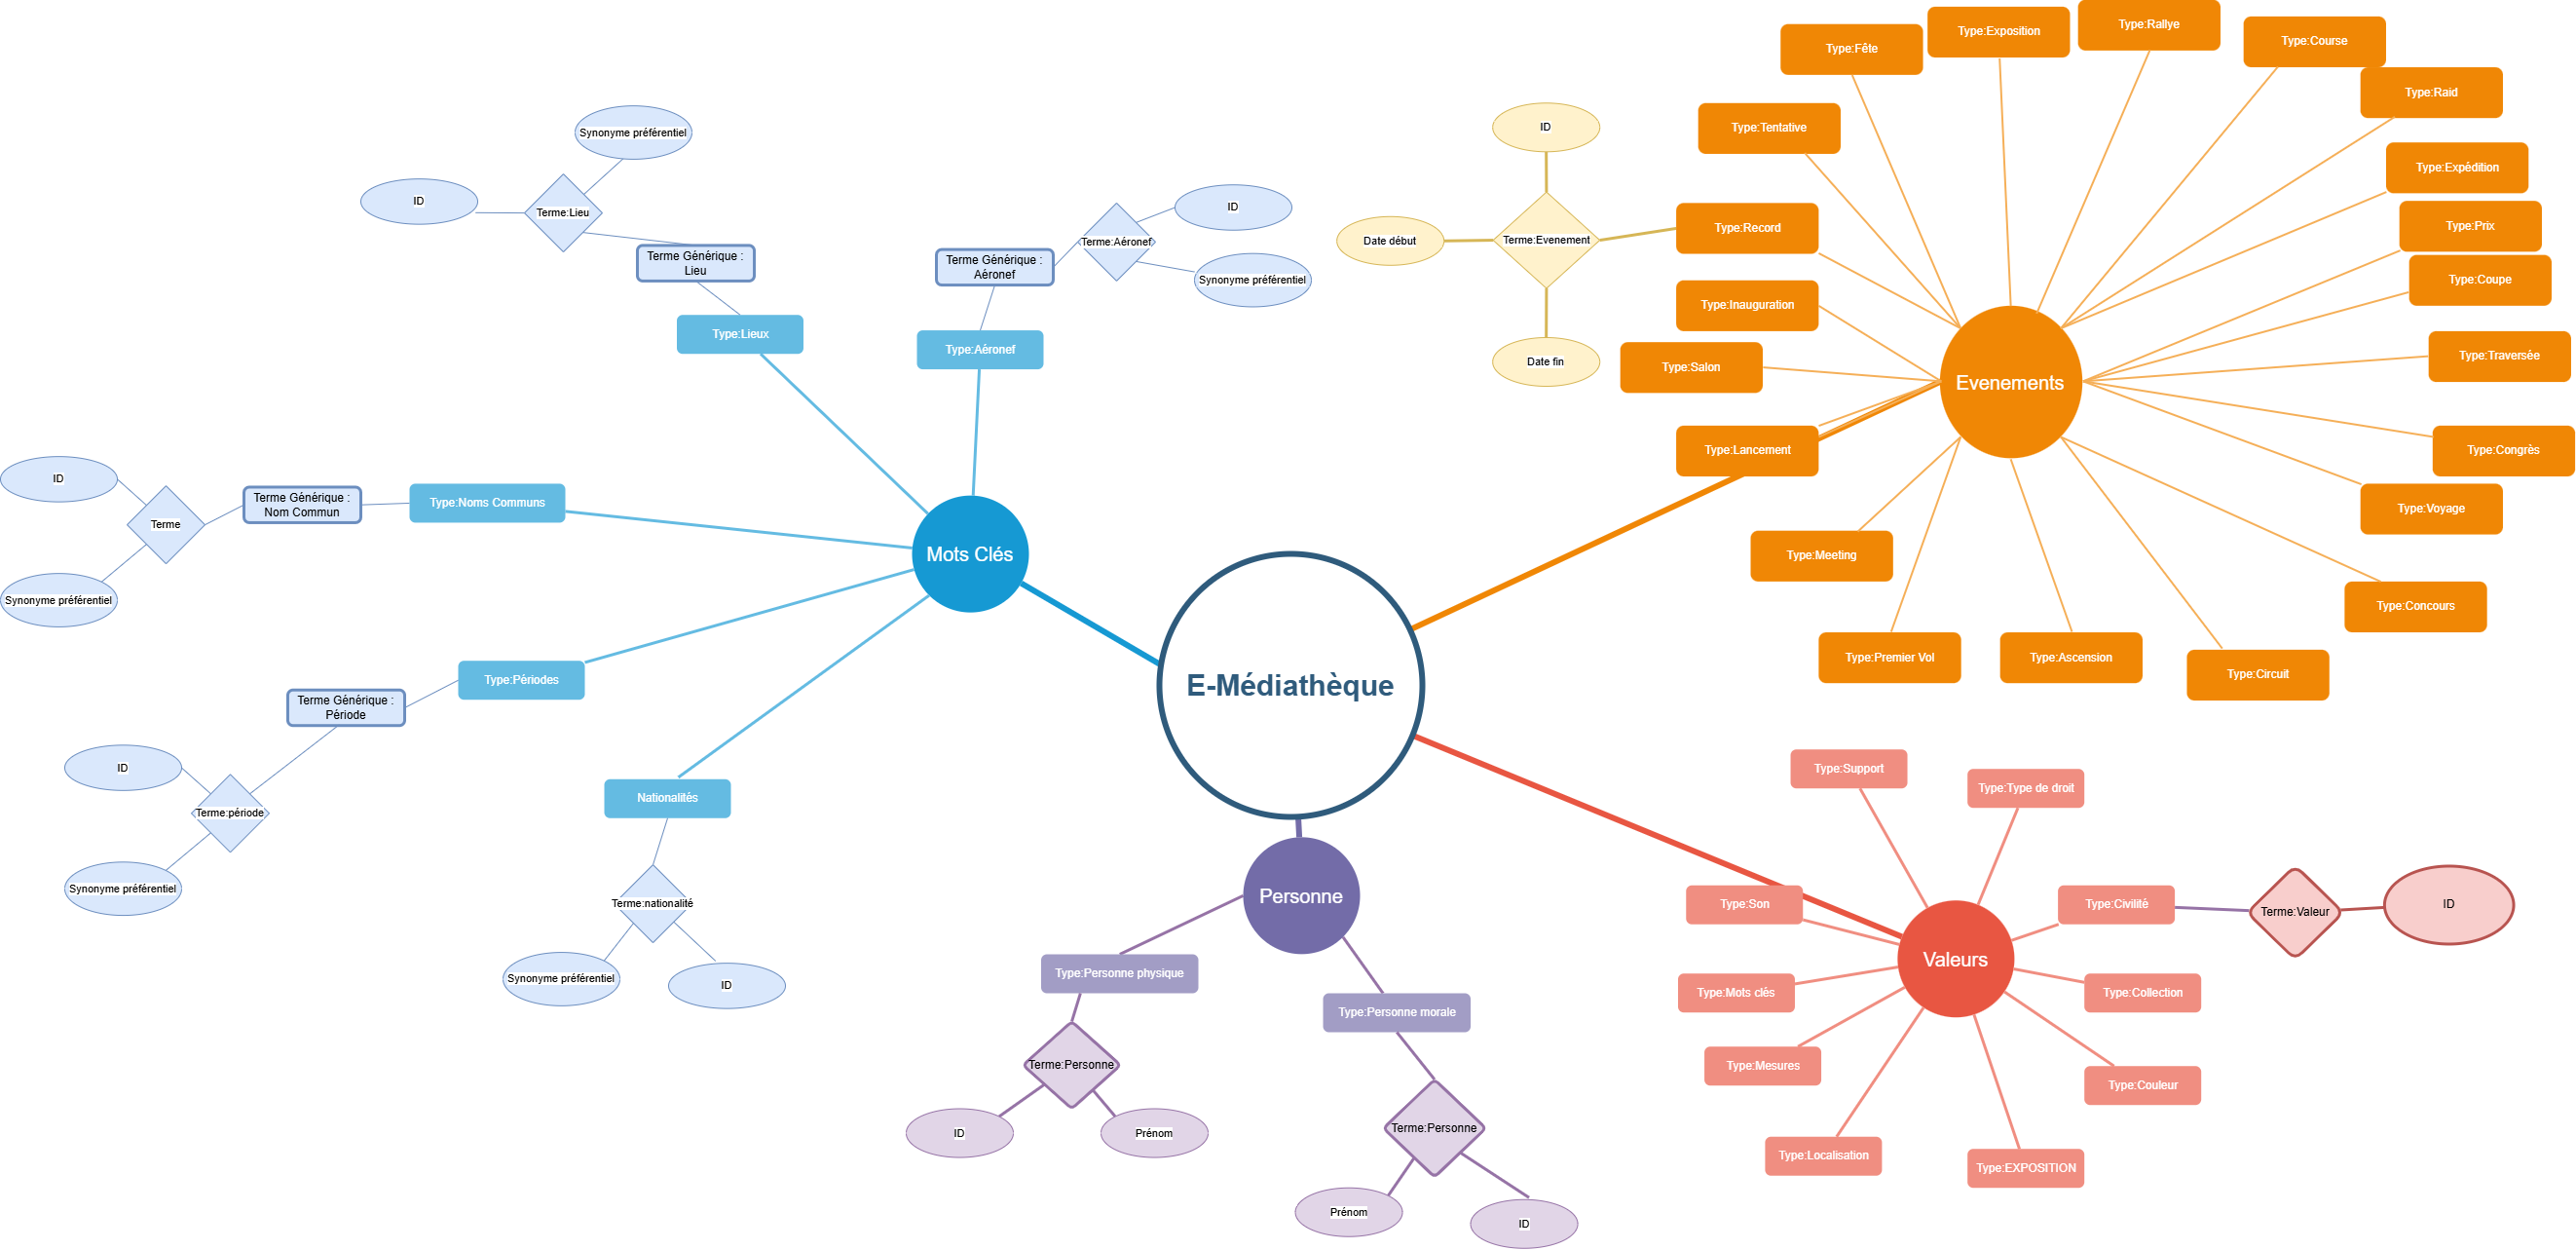
\includegraphics[width=\linewidth]{img/MODEL_emediatheque_mindmap}
		\caption{Modélisation en \textit{mindmap} réalisée avec \textit{draw.io}}
		\label{model:mindmap-emediatheque}
	\end{subfigure}
	\begin{subfigure}{0.35\textwidth}
		\centering
		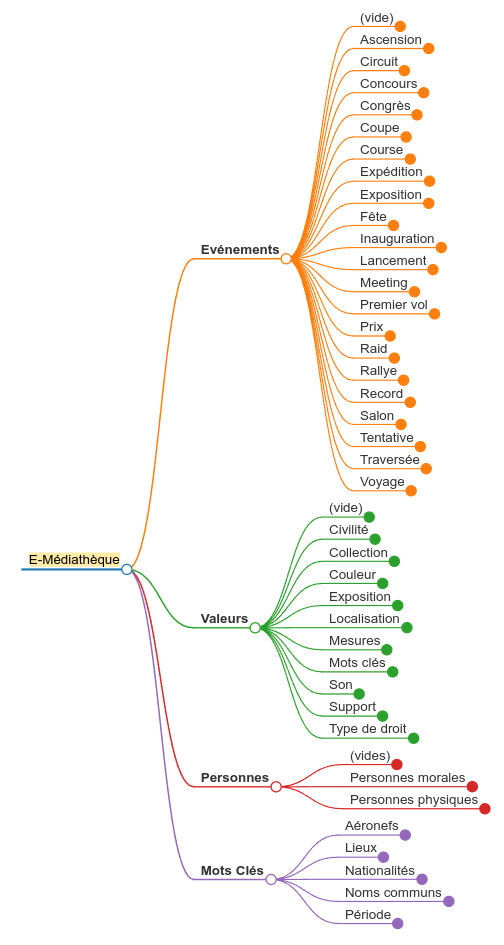
\includegraphics[width=\linewidth]{img/MODEL_emediatheque_arbre}
		\caption{Modélisation en arbre html interactif réalisée avec \textit{markmap}}
		\label{model:arbre-emediatheque}
	\end{subfigure}
	\hfill
	\begin{subfigure}{0.5\textwidth}
		\centering
		\includegraphics[width=\linewidth]{img/GRAPH_emediatheque}
		\caption{Modélisation en graphe réalisée avec \textit{Gephi}}
		\label{model:graph-emediatheque}
	\end{subfigure}
	\caption[Modélisation des \gls{thesaurus} du \mae]{Trois types de modélisations pour un même thésaurus offrent trois approches différentes : notamment, la première permet une vue d'ensemble rapide du type de contenu, la seconde permet d'explorer les branches les unes après les autres, la troisième permet de visualiser des \textit{clusters} de mots -- et pourrait également représenter leurs relations.}
	\label{fig:modelisationthesaurus}
\end{figure}


\paragraph*{Graphes, mindmaps, arbres : l’approche pragmatique}
La visualisation des données par le biais de graphes générés avec Gephi ou d'arbres de concepts interactifs\footnote{Ces arbres, qui auraient également pu être réalisés en Python à l'aide bibliothèques comme \textit{pandas} ou \textit{matplotlib}, ont été réalisés à des fins d'illustration en convertissant un tableau excel en format \textit{markdown} et en générant un fichier html à l'aide de l'application web markmap.} offre une alternative plus intuitive et immédiatement opératoire. Au MAE, ces graphes – qui ont été ensuite mis à disposition de tous les utilisateurs – ont permis de cartographier les clusters thématiques, de détecter les termes orphelins, d'identifier des incohérences dans la hiérarchie des vocabulaires ou des disproportions dans certaines branches du thésaurus. Ils ont servi de support à la restructuration du thésaurus, mais aussi d'outil de médiation entre métiers, lors des groupes de travail ou des ateliers de sensibilisation.

Le format le plus simple -- et donc le plus utilisé, même si moins riche -- a été la modélisation sous forme de \textit{mindmap}, pour représenter seulement les niveaux les plus hauts d'une hiérarchie et travailler sur des grandes catégories de concepts. Celui-ci,  réalisé à partir de logiciels en ligne comme \textit{draw.io}, s'utilise facilement en combinaison avec les tableaux bruts du thésaurus.

On retrouve ici une tension propre à la modélisation documentaire en institution patrimoniale : le compromis entre la formalisation technique – garante de l'interopérabilité et de la pérennité – et la souplesse nécessaire à la prise en main par des agents aux profils variés. Combiner les différents schémas permet ainsi de montrer différents aspects de l'état de l'information au musée, mais aussi de parler à différents profils, et de répondre aux biais, omissions ou transformations inévitables dans toute modélisation et représentation du savoir\footcite{bowkerArrangerChosesConsequences2023}

Ainsi, la modélisation documentaire au \mae~– et plus largement dans les institutions patrimoniales – ne saurait se réduire à un exercice technique. Elle est un instrument de dialogue, d'analyse et de gouvernance, dont la réussite dépend de la capacité à articuler exigence conceptuelle et pragmatisme métier, rigueur des normes et souplesse des usages, pour faire du vocabulaire documentaire un espace partagé, vivant et évolutif.

\begin{table}[htbp]
	\caption{Comparatif des visualisations de données utilisées au MAE pendant le stage}
	\label{tab:comparatif_visualisations}
	\centering
	\setlength{\arrayrulewidth}{0.6pt}
	\renewcommand{\arraystretch}{1.3}
	\begin{tabular}{|p{3cm}|p{4cm}|p{4cm}|p{3cm}|}
		\hline
		\rowcolor{lightgray}
		\textbf{Outil / Visualisation} & \textbf{Avantages principaux} & \textbf{Défauts / Limites} & \textbf{Usages / Destinataires} \\
		\hline
		Diagramme UML & Rigueur, structuration, conformité aux normes (ISO 25964), repérage des écarts avec les standards, interopérabilité forte & Complexité du formalisme, peu accessible pour les non spécialistes, jugé "obscur" & Métiers techniques, experts, audit documentaire \\
		\hline
		Graphe Gephi & Intuitif, interactif, cartographie des clusters, identification des orphelins, support à la restructuration, accessible à tous & Moins formel, difficulté à intégrer des métadonnées complexes, préparation nécessaire & Groupes de travail, ateliers, médiation \\
		\hline
		Arbres de concepts (draw.io, markmap, etc.) & Très accessibles, vues d'ensemble, communication institutionnelle, rapide à réaliser & Peu de granularité, perte de précision sur les liens, adapté aux grandes catégories & Sensibilisation, CA, ateliers \\
		\hline
		Tableaux de synthèse (Excel, markdown) & Utilisation universelle, tri et export rapide, support aux corrections, facile à enrichir & Peu visuel, ne cartographie pas les relations, perte du contexte relationnel & Agents, gestionnaires, formation \\
		\hline
	\end{tabular}
\end{table}

\subsection{La modélisation comme outil de sensibilisation et de pilotage}


La modélisation conceptuelle n’est pas qu’un acte technique : elle est aussi un instrument de sensibilisation et de pilotage institutionnel. Au \mae, l’organisation d’ateliers a permis d’inviter les agents à réfléchir ensemble à la structuration de l’information, à prendre conscience des enjeux de la donnée et de la transmission documentaire.

Ceux-ci ont utilisé la modélisation pour repenser la hiérarchie des termes ou la nomenclature des vocabulaires. Ce travail a permis de concrétiser aux yeux de tous les métiers l'état des connaissances de l'ensemble du musée, et de réfléchir à la manière de les unifier en un unique système.

\bigskip
\bigskip
\bigskip

Ainsi, la modélisation conceptuelle se révèle être le socle sur lequel peut s’édifier une gouvernance documentaire partagée, une culture commune de l’information, et une capacité à piloter le changement dans la durée.

\section{\label{III-A-2}Les solutions techniques existantes : entre standardisation et adaptation locale}


La maîtrise de la prolifération documentaire ne saurait être réduite à une question de modélisation conceptuelle : elle implique le choix raisonné d’outils susceptibles d’articuler la complexité du réel, tout en répondant à des contraintes de gouvernance, d’interopérabilité et de pérennité. Nous nous sommes attachés dans ce mémoire à l'analyse de deux grandes catégories de l'information qui se retrouve dans un musée : celle qui est utilisée pour décrire ses collections, en la matière des thésaurus et vocabulaires contrôlés aujourd'hui présents au musée, et celle qu'il produit quotidiennement dans le cadre de on activité en tant qu'institution publique avec ses archives numériques. Des outils, techniques comme conceptuels, existent pour aider à la structuration et à la diffusion de cette information : nous avons évoqué, pour les archives numérique, l'utilité du respect de normes nationales et d'outils numériques comme une \gls{ged} ou un \ac{sae}. Pour la gestion des vocabulaires contrôlés, c'est un autre outil de modélisation de la connaissance qui s'est imposé : le thésaurus documentaire.



\subsection{\label{III-A-2.1}Qu’est-ce qu’un thésaurus documentaire ?}

On ne peut réduire le thésaurus documentaire à une simple liste de mots ou à un instrument technique. La norme ISO 25964, qui fait aujourd’hui autorité, le définit comme un \enquote{vocabulaire contrôlé et structuré dans lequel les concepts sont représentés par des termes, organisés de façon à ce que des relations entre les concepts soient explicitées, et dont les termes préférentiels sont accompagnés par des entrées vers leurs synonymes ou quasi-synonymes}\footcite{ISO25964120112011,maroyeISO25964Distinction2015}. Celui-ci ne se contente donc pas d’indexer, il articule une vision du monde, une manière de penser le réel à travers le langage documentaire. Il impose donc notamment :
\begin{itemize}
	\item de distinguer le concept (une idée), du terme (le mot choisi pour l'exprimer),
	\item de choisir un terme préféré qui servira à décrire le concept,
	\item de mettre les autres termes en synonymes (\textbf{relations d'équivalence})
	\item des \textbf{relations hiérarchiques} avec :
		\subitem des termes génériques,
		\subitem des termes spécifiques ;
	\item des \textbf{relations d'association} entre les termes,
	\item des définitions, notes et alignements externes associés aux termes.
\end{itemize}

Comme montré dans l'image suivante, la structuration d’un thésaurus suppose ainsi une modélisation précise : chaque concept est relié à des termes, chaque terme préféré est accompagné de notes explicatives, chaque branche de la hiérarchie répond à des logiques de genre à espèce, de tout à partie ou  d'instance à classification\footnote{Pour plus de précisions, consulter l'article suivant \cite{perrinBonnesPratiquesPour2020}}. Cette méthode permet notamment de multiplier les accès à l'information, et de faire entrer en adéquation le langage de l'utilisateur avec le langage de l'institution. 

\begin{figure}
	\centering
	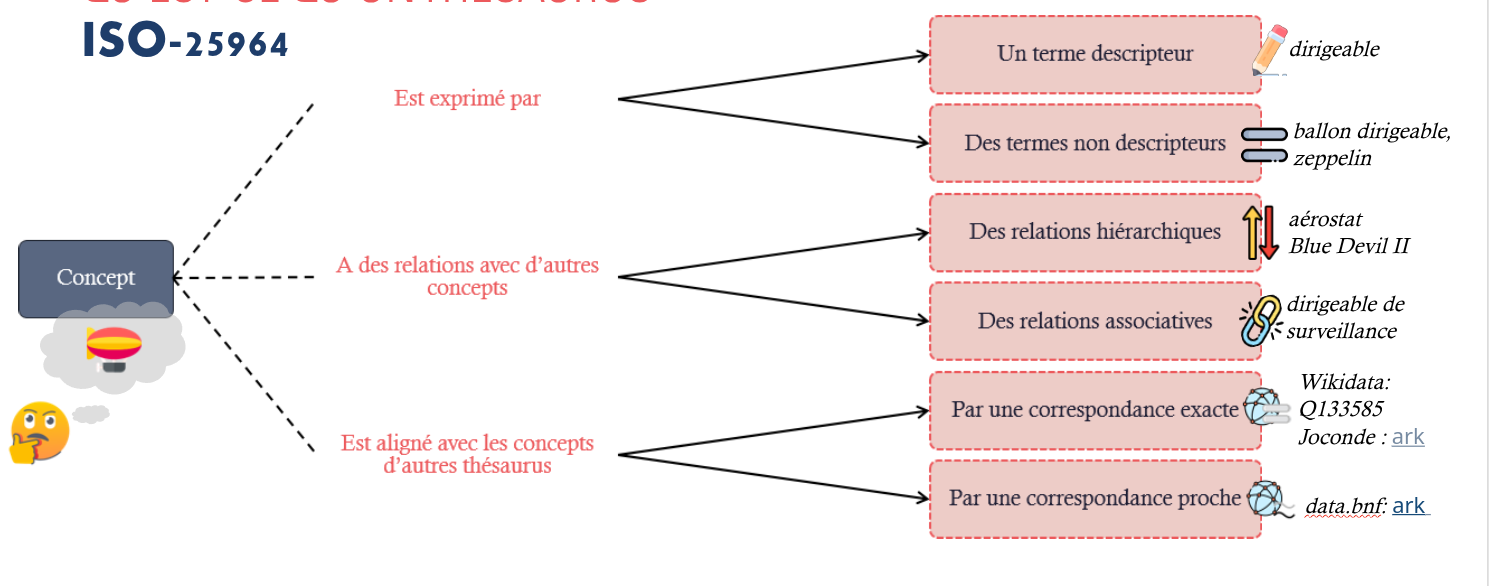
\includegraphics[width=0.9\linewidth]{img/SCHEM_thesaurus}
	\caption[Relations sémantiques exprimées par un thésaurus]{L'ensemble des relations sémantiques exprimées par un thésaurus. \textit{Schéma utilisé dans la formation du 4 juin 2025, inspiré de \protect\cite{perrinBonnesPratiquesPour2020}}.}
	\label{fig:schemthesaurus}
\end{figure}


\subsection{Diversité des outils de structuration de l’information}

Simple et efficace, le \gls{thesaurus} s'est imposé au \mae comme un outil compatible avec les logiciels métiers utilisés. Au fil des réflexions sur leur réorganisation, sont cependant apparues diverses difficultés : il est en effet apparu que le \gls{thesaurus} ne permettrait pas d'englober l'ensemble des connaissances requises au musée pour gérer ses collections. En effet, un thésaurus reste un outil lexical, qui permet de contrôler la description des objets : il ne permet pas, par exemple, de symboliser des liens de famille entre des personnes enregistrées comme terme ou d'expliciter les types de relations -- auteur, constructeur, utilisé dans... -- entre deux termes associés.
Il est apparu que pour arriver à cette granularité d'information, un autre outil devrait être adopté : l'ontologie documentaire. Pour citer Thomas Francart, expert dans les systèmes de gestion des connaissances et fondateur de la société SPARNA, \blockquote{l’ontologie cherche à décrire de façon formelle un domaine de connaissance, en identifiant les types d’objets de ce domaine, leurs propriétés et leurs relations\footcite{francartOntologieThesaurusTaxonomie2013}.}

Bien plus riche que le thésaurus, ce format pourrait répondre aux besoins diversifiés du \mae en lui permettant de couvrir davantage de connaissances, et de mieux adresser la diversité de ses utilisateurs avec un système plus modulables que le thésaurus : sa mise en place demanderait cependant un travail de restructuration, de recherche et de création de liens considérable.

C'est le choix qui a été fait par d'autres institutions devant répondre à des exigences similaires : pour ne pas citer le cas bien connu de la \ac{bnf}, citons par exemple celui de la fondation SAPA -- Archives suisses des arts de la scène qui a migré en 2021 toutes les métadonnées de ses collections en une ontologie utilisant le nouveau standard de description \ac{rdf} \ac{rico}\footnote{Sur \ac{rico}, voir \cite{bruleauxRecordsContextsRIC2024}}. Ce format d'ontologie documentaire lui permet ainsi une granularité extrême et une interopérabilité native avec les standards du web sémantique\footcite{coulonDeploiementNormeRecords2024} : l'auteur insiste cependant sur sa nouveauté, l'absence d'une communauté active pour aider à la mise en place du système, et d'outils informatiques appropriés. Il insiste fortement sur \enquote{le bouleversement de nos pratiques professionnelles qui dépasse la nouvelle norme en elle-même} qu'a apporté la migration, montrant que ce type de projet, bien qu'il aboutisse à un système finalement robuste et efficace pour partager et dépasser les \enquote{silos} de données, demande à l'institution qui le met en place un investissement considérable de temps et de ressources, une familiarisation à ces nouvelles techniques, et exige enfin d'être prêt à changer la manière de travailler de l'ensemble de ses utilisateurs.

\subsection{Solutions pour l’interopérabilité et l’ouverture}

L’histoire des normes documentaires, à ce titre, est celle d’une lente montée en exigence : du premier standard Z39.19, consacré à la structuration des thésaurus pour la recherche documentaire, à la norme ISO 25964 publiée en 2011, qui impose la distinction concept/terme et formalise les relations hiérarchiques, associatives et d’équivalence, chaque étape marque un progrès vers la mise en dialogue des systèmes. Comme le souligne Dominique Chichereau, le mouvement de normalisation des thésaurus qui s'est amorcé dès les années 1970 a accompagné le développement de l’informatisation documentaire , et s’est accéléré avec l’essor du web sémantique et la nécessité d'interopérabilité entre des vocabulaires hétérogènes\footcite{chichereauNormesConceptionGestion2007}.

[TODO : schéma d'explication skos rdf ou ajout au glossaire]
C’est dans ce contexte qu'est apparu \ac{skos}, publié par le \ac{w3c} pour \enquote{proposer un système permettant d’exprimer et de gérer des modèles interprétables par les machines dans la perspective du web sémantique\footcite{lenartSKOSLangageRepresentation2007}}, en offrant un modèle fondé sur des triplets \ac{rdf}. Ce standard permet notamment de décrire les concepts, leurs labels multilingues, et les relations hiérarchiques ou associatives entre eux.  \ac{skos} s’impose dès lors comme un langage technique idéal,\enquote{défini comme « simple » par opposition à d’autres modèles, comme OWL (Ontologic Web Language)}, pour mutualiser les vocabulaires sur le web tout en respectant la complexité des relations et la richesse des annotations. 

Bien qu'il existe d'autres solutions de gestion du vocabulaire et que l'avènement de l'intelligence artificielle pousse des institutions à se tourner vers des modèles plus complexes pour implémenter des solutions IA, de la Bibliothèque nationale de Finlande, qui expose ses vocabulaires sur Skosmos\footcite{Skosmos} également utilisé pour le thésaurus de l’UNESCO\footcite{unescoThesaurusLUNESCO1977}, en passant par des institutions patrimoniales françaises telles que le ministère de la Culture avec le thésaurus de Joconde\footcite{ministeredelacultureListeDautoriteDenomination} ou le réseau \ac{frantiq}\footcite{Pactols}, l’usage du format \ac{skos} pour la structuration et la diffusion de thésaurus s’est aujourd’hui imposé aussi bien dans le monde de la recherche, de l’administration publique que dans l’écosystème documentaire des grands musées.
	
	
L’avènement de \ac{skos} et la généralisation du web sémantique n’ont pas seulement permis d’exposer les vocabulaires : ils ont ouvert la voie à une ambition nouvelle, celle de l’alignement des données, qui consacre la possibilité pour chaque institution de faire dialoguer ses savoirs avec ceux de ses pairs. Aligner en effet, c'est relier explicitement des concepts équivalents ou proches, structurer leurs correspondances à l’aide des propriétés (en \ac{skos}, \lstinline|skos:exactMatch|, \lstinline|closeMatch|, \lstinline|broadMatch| ou \lstinline|related|). Ce travail, loin d’être purement technique, engage une réflexion sur la valeur des termes, la portée des synonymes et la fidélité aux usages locaux : il impose de choisir, parmi la profusion des vocabulaires, ceux qui feront pont entre les systèmes et permettront la circulation des connaissances. Au \mae -- ou il n'est encore qu'à l'état de projet -- comme ailleurs, l’alignement avec les thésaurus de Joconde, le SUDOC ou Wikidata ne se réduit pas à un échange de fichiers : il suppose une révision minutieuse des branches, une concertation des acteurs, une vigilance sur les notes historiques et les spécificités des collections. Cette opération apparaît ainsi comme le prolongement naturel de toute politique documentaire soucieuse d’ouverture et de pérennité, pour garantir à l'institution sa capacité à se transmettre, à s’enrichir, et à dialoguer au sein d’un univers patrimonial interconnecté.

\section{\label{III-A-3}L’intégration dans l’écosystème institutionnel : vers une gouvernance collaborative des outils}

L’intégration du logiciel Opentheso au \mae~semblerait être la solution qui réponde le mieux à ses aspirations de gouvernance du vocabulaire et d'interopérabilité avec le web. Cet outil libre recommandé par le ministère de la Culture, s’impose aujourd'hui en France comme le socle d’un vocabulaire  capable de transcender les cloisonnements logiciels et de fédérer les métiers. Sa conformité aux normes ISO 25964 et au standard \gls{skos}, sa capacité à exporter dans des formats interopérables \gls{rdf}, comme \textit{Turtle} ou \textit{JSON-LD}, à visualiser l’arborescence en graphe, à documenter les relations synonymiques ou hiérarchiques, en font un instrument rigoureux qui peut être au service à la fois de la recherche et de la médiation. Opentheso permet de structurer la connaissance, mais aussi de relier les bases métiers – un plugin d'intégration dans \gls{koha} existe déjà, et il serait envisageable de demander une intégration à \textit{Skinsoft} pour Archange qui permettrait au logiciel d'interagir avec l'\ac{api} d'OpenTheso.

La mise en place, en complément, d'un réseau de logiciels dédiés à une gestion rationalisée de l'information au \mae~-- comme des versements réguliers sur le \gls{sae} Vitam pour l’archivage et la mise en place d'une \gls{ged} – serait d'une grande aide au musée pour parvenir à ses ambitions de gouvernance.

\subsection{Accompagnement au changement et formation des agents}

Toute réforme documentaire ne pourra cependant aboutir sans accompagnement au changement : ateliers de sensibilisation, guides d’usage, fresques de la connaissance, tutoriels, autant de dispositifs qui harmoniseraient les pratiques et préparent les agents à la prise en main des nouveaux outils. La formation s'imposera comme la condition de la réussite : elle permettra de comprendre la logique des outils, de s’approprier les méthodes de structuration et d’assurer la pérennité des acquis.

\subsection{Interopérabilité et dialogue intermétiers}

L’interopérabilité enfin, même si la mise en place de solutions dédiées l'aidera grandement, ne se limitera pas à la technique : elle suppose un dialogue continu entre les métiers du musée et une construction de passerelles entre les silos professionnels et plateformes. Les groupes de travail menés au musée ont permis de réfléchir à des solutions communes pour l’archivage numérique et l'unification des thésaurus, ils devront continuer pour les mettre en place et assurer leur bon fonctionnement. 


\bigskip
\bigskip
\bigskip

\lettrine{A}insi se dessine, à travers l’expérience du Musée de l’Air et de l’Espace, une voie exigeante pour la maîtrise de la prolifération documentaire. Il ne s’agit pas seulement de juxtaposer modèles conceptuels, outils techniques et dispositifs de gouvernance : il faut les articuler, les penser ensemble, dans une logique de préservation de la richesse sémantique et d’ouverture à l’interopérabilité. Les solutions expérimentées — modélisation via Gephi, migration vers Opentheso, ateliers de sensibilisation, harmonisation documentaire — illustrent la nécessité d’allier rigueur, adaptation et accompagnement au changement pour garantir la transmission du patrimoine et la vitalité de l’écosystème muséal.